% paper/sections/11b_spatial_geometry.tex
% ─────────────────────────────────────────────────────────────────────────────
\subsubsection{\texorpdfstring{曲率計算の格子収束}{曲率計算の格子収束}}
\label{sec:verify_curvature}
% ─────────────────────────────────────────────────────────────────────────────

\noindent\textbf{目的：}
CSF における曲率 $\kappa$（式~\eqref{eq:curvature_2d}）の実装精度を，
円形界面および正弦波状界面の製造解で検証する．
本テストは CCD 演算子の全成分
\[
  D_x^{(10)},\quad D_y^{(01)},\quad
  D_{xx}^{(20)},\quad D_{yy}^{(02)},\quad D_{xy}^{(11)}
\]
を含む曲率計算経路の総合誤差を測定する．

\noindent\textbf{評価対象：}
CLS 変数 $\psi$ から計算される CCD 曲率
（\texttt{CurvatureCalculator.compute}）と，
比較用の 2 次中心差分（CD2）曲率．

\noindent\textbf{手順とパラメタ：}
曲率は
$\kappa = -(\phi_{xx}\phi_y^2 - 2\phi_{xy}\phi_x\phi_y + \phi_{yy}\phi_x^2)/|\bnabla\phi|^3$
に対応する式を用いて計算される．テスト問題は次の 2 つである：
\begin{itemize}[noitemsep]
  \item 円形界面：$R=0.25$，$\kappa_{\mathrm{exact}} = 4$，
        CCD 曲率と CD2 曲率を比較する．
  \item 正弦波状界面：$y = 0.5 + 0.05\sin(2\pi x)$，
        解析解 $\kappa = -f''/(1+f'^2)^{3/2}$ と CCD 曲率を比較する．
\end{itemize}
いずれも $\varepsilon = 1.5h$，評価帯は $|\phi| < 3h$ とし，
評価指標は $L_\infty$ 誤差と収束次数である．

\noindent\textbf{結果：}

\begin{table}[htbp]
\centering
\caption{円形界面の曲率 $L_\infty$ 誤差収束：
  CCD 曲率 vs CD2 曲率（$R=0.25$，$\varepsilon = 1.5h$）}
\label{tab:curvature_circle}
\renewcommand{\arraystretch}{1.3}
\begin{tabular}{rrrrr}
\toprule
$N$ & CCD 誤差 & 次数 & CD2 誤差 & 次数 \\
\midrule
 16 & $8.93 \times 10^{0}$ & ---  & $8.82 \times 10^{0}$ & ---  \\
 32 & $2.34 \times 10^{0}$ & 1.93 & $2.23 \times 10^{0}$ & 1.98 \\
 64 & $9.09 \times 10^{-1}$ & 1.36 & $9.12 \times 10^{-1}$ & 1.29 \\
128 & $4.11 \times 10^{-1}$ & 1.14 & $4.10 \times 10^{-1}$ & 1.15 \\
256 & $1.96 \times 10^{-1}$ & 1.07 & $1.96 \times 10^{-1}$ & 1.07 \\
\bottomrule
\end{tabular}
\end{table}

\begin{table}[htbp]
\centering
\caption{正弦波状界面の CCD 曲率 $L_\infty$ 誤差収束
  （$A = 0.05$，$\varepsilon = 1.5h$）}
\label{tab:curvature_sinusoidal}
\renewcommand{\arraystretch}{1.3}
\begin{tabular}{rrr}
\toprule
$N$ & CCD 誤差 & 次数 \\
\midrule
 32 & $1.60 \times 10^{-2}$ & ---  \\
 64 & $8.38 \times 10^{-3}$ & 0.93 \\
128 & $4.22 \times 10^{-3}$ & 0.99 \\
256 & $2.13 \times 10^{-3}$ & 0.99 \\
\bottomrule
\end{tabular}
\end{table}

円形界面では CCD 曲率と CD2 曲率がほぼ同じ誤差水準を示し，
$L_\infty$ 収束は漸近的に $\Ord{h^1}$ 程度である．
これは評価帯を $|\phi|<3h$ とし，かつ界面厚みを
$\varepsilon = 1.5h$ としているため，正則化された CLS 曲率の誤差が
離散微分の形式次数より先に支配的になることを示す．
正弦波状界面でも $L_\infty$ 誤差は単調減少するが，
実測次数は約 $\Ord{h^1}$ にとどまる．
したがって本テストは CCD 微分演算子単体の高次精度ではなく，
CLS 正則化幅を含む現行曲率パイプラインの実効精度を評価するものと位置づける．
CCD 微分演算子単体の設計精度は §~\ref{sec:verify_ccd_convergence} および
§~\ref{sec:verify_mixed_partial} で別途確認する．

\begin{figure}[htbp]
\centering
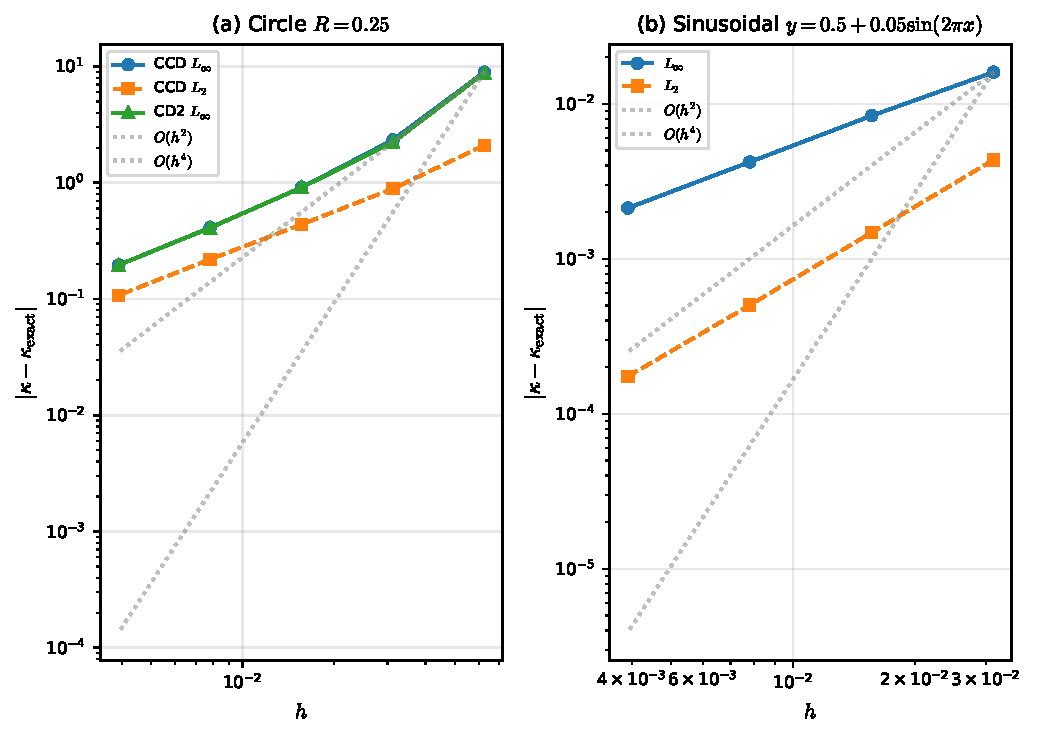
\includegraphics[width=0.92\linewidth]{figures/ch11_curvature_3path}
\caption{曲率 $\kappa$ の格子収束．
  (a) 円形界面（$R=0.25$）：CCD 曲率と CD2 曲率の比較．
  (b) 正弦波状界面：CCD 曲率の格子収束．}
\label{fig:curvature_3path}
\end{figure}

\noindent\textbf{結論：}
現行の CLS 曲率パイプラインは円形・正弦波状界面の双方で誤差を単調に減少させるが，
$L_\infty$ 実効次数は約 $\Ord{h^1}$ であり，
正則化幅 $\varepsilon=\Ord{h}$ と界面近傍評価帯が精度を律速する．
本節の結果は曲率パイプラインの実効精度評価であり，
CCD 演算子単体の $\Ord{h^5}$--$\Ord{h^6}$ 精度を主張する根拠としては用いない．

% ─────────────────────────────────────────────────────────────────────────────
\subsubsection{Rhie--Chow 補正の高次精度化}
\label{sec:verify_rc_bracket}
% ─────────────────────────────────────────────────────────────────────────────

\noindent\textbf{目的：}
§~\ref{sec:rc_high_order} で導出した C/RC（CCD-enhanced RC）ブラケットが
$\Ord{h^4}$ を達成することを検証する．

\noindent\textbf{評価対象：}
RC ブラケット：標準 RC（$\Ord{h^2}$，式~\eqref{eq:rc_detection_taylor}）
vs C/RC（$\Ord{h^4}$，式~\eqref{eq:rc_crc_bracket}）．

\noindent\textbf{手順とパラメタ：}
\begin{itemize}[noitemsep]
  \item テスト関数 $p = \cos(2\pi x)\cos(2\pi y)$（$p'''$ が解析的に既知）
  \item 周期境界条件，格子 $N = 16, 32, 64, 128$
  \item 各フェイスにおける標準ブラケットと C/RC ブラケットの $L^\infty$ 誤差を計測
\end{itemize}

\noindent\textbf{結果：}

\begin{table}[htbp]
\centering
\caption{RC ブラケットの格子収束：標準 RC（$\Ord{h^2}$）vs C/RC（$\Ord{h^4}$）}
\label{tab:rc_bracket_convergence}
\renewcommand{\arraystretch}{1.3}
\begin{tabular}{rccccr}
\toprule
$N$ & $\|\text{std}\|_\infty$ & 次数 & $\|\text{C/RC}\|_\infty$ & 次数 & 改善倍率 \\
\midrule
 16 & $3.95 \times 10^{-2}$ & ---  & $1.78 \times 10^{-4}$ & ---  & $222\times$ \\
 32 & $1.00 \times 10^{-2}$ & 1.98 & $1.13 \times 10^{-5}$ & 3.98 & $889\times$ \\
 64 & $2.52 \times 10^{-3}$ & 1.99 & $7.08 \times 10^{-7}$ & 3.99 & $3557\times$ \\
128 & $6.31 \times 10^{-4}$ & 2.00 & $4.43 \times 10^{-8}$ & 4.00 & $14229\times$ \\
\bottomrule
\end{tabular}
\end{table}

標準 RC は理論通り $\Ord{h^2}$ で収束し，
C/RC は正確に $\Ord{h^4}$ を達成した（表~\ref{tab:rc_bracket_convergence}）．
$N = 128$ において C/RC は標準比約 14000 倍の改善を示す．
CCD は 1 回の求解で $p'$ と $p''$ を同時に返すため，
C/RC の実装に\textbf{追加の CCD 呼び出しは一切不要}である．
この「ゼロコスト」の精度改善は，CCD の同時微分出力という設計特性に固有の利点であり，
従来の有限差分法や有限体積法では実現できない．
図~\ref{fig:rc_bracket} に収束曲線を示す．

\begin{figure}[htbp]
\centering
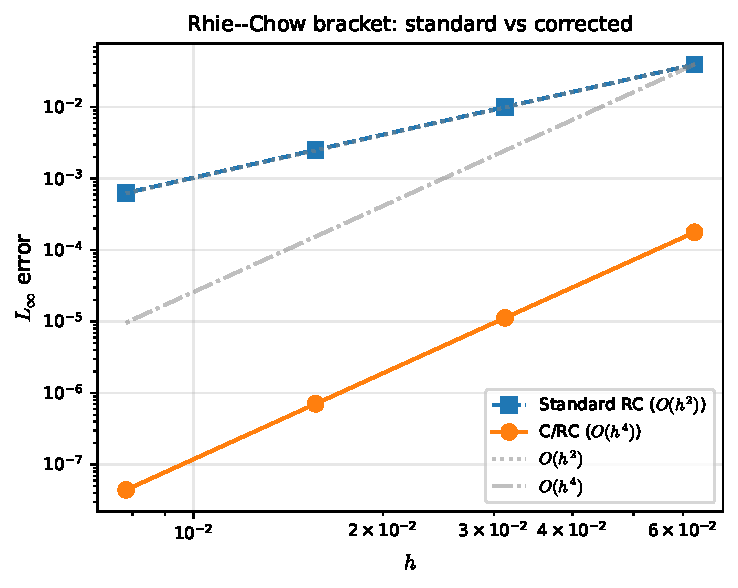
\includegraphics[width=0.88\linewidth]{figures/ch11_rc_bracket}
\caption{RC ブラケット格子収束：標準 RC（$\Ord{h^2}$）vs C/RC（$\Ord{h^4}$）．
  C/RC は CCD が同時計算する $p''$ のみを利用し，
  $N=128$ で標準比約 14000 倍の精度を達成する．}
\label{fig:rc_bracket}
\end{figure}

\noindent\textbf{結論：}
C/RC は正確に $\Ord{h^4}$ を達成し，$N = 128$ で標準比約 14000 倍の改善を示す．
CCD は 1 回の求解で $p'$ と $p''$ を同時に返すため，
追加の CCD 呼び出しは一切不要（ゼロコスト精度改善）である．

% ─────────────────────────────────────────────────────────────────────────────
\subsubsection{2D 混合偏微分の CCD 精度}
\label{sec:verify_mixed_partial}
% ─────────────────────────────────────────────────────────────────────────────

§~\ref{sec:ccd_metric} で述べた逐次 CCD 適用による
混合偏微分 $\partial^2 f / \partial x \partial y$ の精度を検証する．
テスト関数 $f(x,y) = \sin(2\pi x)\cos(2\pi y)$
（厳密解 $f_{xy} = -4\pi^2 \cos(2\pi x)\sin(2\pi y)$）に対し，
$\partial_x \to \partial_y$ と $\partial_y \to \partial_x$ の両順序で
$L_\infty$ 誤差と収束次数を測定した（$N = 16$--$256$）．

\begin{table}[htbp]
\centering
\caption{混合偏微分 $\partial^2 f / \partial x \partial y$ の格子収束}
\label{tab:mixed_partial}
\renewcommand{\arraystretch}{1.2}
\small
\begin{tabular}{rcccc}
\toprule
$N$ & $L_\infty$（周期） & 次数 & $L_\infty$（壁） & 次数 \\
\midrule
 16 & $3.23 \times 10^{-5}$ & ---  & $3.59 \times 10^{-3}$ & --- \\
 32 & $4.85 \times 10^{-7}$ & 6.06 & $1.12 \times 10^{-4}$ & 5.01 \\
 64 & $7.51 \times 10^{-9}$ & 6.01 & $3.79 \times 10^{-6}$ & 4.88 \\
128 & $1.18 \times 10^{-10}$ & 6.00 & $1.21 \times 10^{-7}$ & 4.97 \\
256 & $1.50 \times 10^{-11}$ & 2.97\textsuperscript{*} & $3.80 \times 10^{-9}$ & 4.99 \\
\bottomrule
\multicolumn{5}{l}{\footnotesize \textsuperscript{*}$N{=}256$ は丸め誤差到達．} \\
\end{tabular}
\end{table}

適用順序の交換による誤差（可換性誤差）は全条件で $\Ord{10^{-12}}$ 以下であり，
演算子の可換性が機械精度で成立している．

\noindent\textbf{結論：}
逐次 CCD 適用による混合偏微分は周期境界で $\Ord{h^{6.0}}$，
壁境界で $\Ord{h^{5.0}}$（境界スキーム律速）を達成した．
これは非対角粘性項 $\partial_y(\mu\,\partial_x u)$ の離散化に
必要な精度要件を満たしている．
